\documentclass[10pt]{article}
\usepackage[]{ragged2e}
\usepackage{fancyhdr,amsmath,amsthm,amssymb,bbm,graphicx,array,bm,tensor,braket,mathtools}
\usepackage{mathtools,tkz-euclide}
\usepackage[utf8]{inputenc}
\usepackage[letterpaper,left=25mm,right=25mm]{geometry}

\setlength{\parskip}{1em}
\setlength{\parindent}{0em}

\newcommand{\Z}{\mathbb{Z}}
\newcommand{\R}{\mathbb{R}}
\newcommand{\Q}{\mathbb{Q}}
\newcommand{\C}{\mathbb{C}}
\newcommand{\N}{\mathbb{N}}

\DeclareMathOperator{\Ima}{Im}

\linespread{1.25}
\pagestyle{fancy}
\fancyhf{}
\lhead{PHYS 825 $|$  Assignment 2}

\rhead{Dilraj Ghuman $|$ 20191345}

\begin{document}

\textbf{\Large 1. Dimensional Analysis}

\textbf{Q1} \textit{Derive the relationship between the period of a pendulum, gravitational accelera-
tion, and the pendulum’s relevant physical quantities.}

Simple exercise of comparing dimensions. In particular we know that period, $P \sim [T]$, must be related to the two physical quantities of gravity, $g \sim [L][T]^{-2}$, and length of the string, $\ell \sim [L]$. Thus, supposing some constant, $\alpha$, we can suppose

\begin{align*}
  P & \sim \alpha g^{a}\ell^{b} \sim \alpha\left([L][T]^{-2}\right)^{a}[L]^{b} \\
  [T] & \sim \alpha [L]^{a + c}[T]^{-2a} 
\end{align*}
\[
\implies a = -\frac{1}{2} \hspace{2em} \implies \hspace{2em} b = \frac{1}{2}
\]
and thus, $P \sim \alpha\sqrt{\frac{\ell}{g}}$.

\textbf{Q2} \textit{Beginning only with the knowledge that a right triangle’s area is some function of
the length of its hypotenuse and a non-right adjoining angle, prove the Pythagorean
theorem using dimensional analysis. (Do not use any trigonometric identities. You
may use basic geometry. The standard solution involves drawing a certain line that
splits the right triangle into smaller right triangles.)}

We start by splitting our right angle triangle into two parts:

\begin{center}
  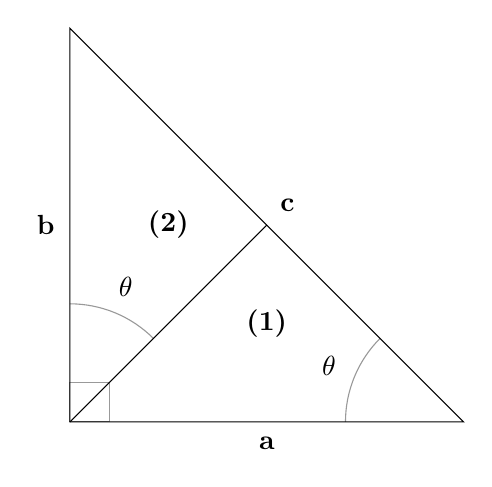
\begin{tikzpicture}[scale=5]
    % Define Edges
    \coordinate (A) at (0,0);
    \coordinate (B) at (1,0);
    \coordinate (C) at (0,1);
    \coordinate (D) at (0.5,0.5);
    % Cycle through
    \draw (A)--(B)--(C)--cycle;
    % Bisection
    \draw (0,0) -- (0.5,0.5);
    % Labels
    \tkzLabelSegment[below=2pt](A,B){\textbf{a}}
    \tkzLabelSegment[left=2pt](A,C){\textbf{b}}
    \tkzLabelSegment[above right=2pt](B,C){\textbf{c}}
    % Label Sections
    \node at (0.5,0.25) {\textbf{(1)}};
    \node at (0.25,0.5) {\textbf{(2)}};
    % Angles
    \tkzMarkRightAngle[fill=none,size=0.1,opacity=.4](C,A,B)
    \tkzMarkAngle[fill=none,size=0.3,opacity=.4](C,B,A)
    \tkzMarkAngle[fill=none,size=0.3,opacity=.4](D,A,C)
    \tkzLabelAngle[pos = 0.37](C,B,A){\(\theta\)}
    \tkzLabelAngle[pos = 0.37](D,A,C){\(\theta\)}
  \end{tikzpicture}
\end{center}

Note by geometric properties, the two smaller triangles (\textbf{(1)} and \textbf{(2)}) are actually similar (infact, all 3 are similar!). Thus, as is shown with $\theta$ being consistent with them both, we can apply our rule of area:

\[
\begin{aligned}
  A_{(0)} & = A_{(1)} + A_{(2)} \\
  c^{2}f(\theta) & = a^{2}f(\theta) + b^{2}f(\theta) \\
  \Aboxed{c^{2} & = a^{2} + b^{2}}
\end{aligned}
\]

\textbf{Q3} \textit{Derive the relationship between the number of rowers in a boat, and the boat’s speed. Assume each rower contributes the same power to the boat’s motion. (Hint:The drag force the rowers are pulling against is given by $F \sim \rho A v^{2}$, where $\rho$ is the density of water and $A$ is the area of a boat. Archimedes’ principle of displacement should inform you as to how $A$ changes with the number of rowers.)}

First, we need to relate the number of rowers with the area of the boat, $A$. This effectively reduces to the square-cubed law; the depth of the boat scales with $n$ so the area must go as $a^{\frac{2}{3}}$. Now, the problem is straight forward if we assume maximum velocity of the boat:
\[
\begin{aligned}
  F & \sim \rho Av^{2} \\
  P & \sim \rho a^{\frac{2}{3}}v^{3} \\
  n & \sim \rho a^{\frac{2}{3}}v^{3} \\
  \Aboxed{v & \sim n^{\frac{1}{9}}\rho^{-\frac{1}{3}}}
\end{aligned}
\]

\textbf{Q4} \textit{Srednicki 12.3}

This is simple; we know that distance is inversely proportional to mass in natural units, so we can approximate $r$ as such:
\[ r \sim \frac{1}{m} = \frac{1}{0.938\, \text{GeV}}\cdot 2\times10^{-14}\,\text{Gev}\cdot\text{cm} = 2.132\times10^{-14}\,\text{cm} \]
as required.

\textbf{\Large 2. Ising Model}

\textbf{Q1} \textit{The nearest neighbor Ising model has a certain “$Z_{2}$ symmetry” sometimes called the Ising model time symmetry. Prove that the nearest neighbor Ising model free energy density is invariant under the replacement $B \to -B$. (Note that the free energy density here is defined for a very large or infinite Ising model system). Say as plainly as you can why the nearest neighbor Ising model has this symmetry.}

We first look at the energy equation to see how it transforms when we $B \to -B$:
\[
E \to E' = -(-B)\sum_{i}s_{i} - J\sum_{\langle ij\rangle}s_{i}s_{j} = -B\sum_{i}(-s_{i}) - J\sum_{\langle ij\rangle}s_{i}s_{j} 
\]
\[
E\to E' = s_{i} \to -s_{i} \, .
\]

So, in our free energy equation, we see
\[
F \to F' = -T\log Z' = -T\log\left(\sum_{\{s_{i}\}}e^{-\beta E'}\right)
\]
but we know that
\[
\sum_{\{s_{i}\}}f(s_{i}) = \sum_{\{s_{i}\}}f(-s_{i})
\]
so it must be true that $F \to F' = F$, and hence the free energy is invariant under this transformation. Physically, this is saying that we can flip the magnetic field but the average free energy in the system will remain unchanged. This makes sense, we don't add energy by choosing a different direction for the magnetic field!

\textbf{Q2} \textit{The nearest neighbor Ising model has an additional symmetry for $B = 0$. For this case of zero external magnetic field, there is an additional symmetry of the free energy density under the replacement $J \to -J$, so long as the Ising model is defined over a cubic [3d] (or square [2d] or linear [1d]) tiled lattice. To prove this, you will want to first define interlocking sub-lattices of the Ising model, $a$ and $b$, such that $a$'s have only $b$'s adjacent to them, and $b$'s have only $a$'s adjacent to them. For example for the linear case this is easy, every other site is labeled $a$, the rest $b$. Say as plainly as you can why the nearest neighbor Ising model has this symmetry, only when $B = 0$.}

We can show this transformation is equivalent to another, just like above. In particular, we start by partitioning our set into the $a$'s and $b$'s. In particular, it is easy to imagine we can define these sub-lattices, by first starting with the linear case; we just alternate between $a$'s and $b$'s. For the 2D case, we can imagine alternating between each layer and building up the sheet. For the 3D case we repeat this method to produce a 3D lattice.

Now that we know these sub-lattices do indeed exist, atleast for the 1, 2 and 3 dimensional cases, we can move onto the transformation. To start, we note that since the $J$ coupling only pairs nearest neighbours, we can rewrite the energy as
\[
E = -J\sum_{\langle ij\rangle}s_{i}s_{j} = -J\sum_{\langle ij\rangle}s^{A}_{i}s^{B}_{j}
\]
where $s^{A}_{i}$ is in the $a$'s and $s^{B}_{j}$ is in the $b$'s. In this case, as in \textbf{Q1}, we can apply the transformation and see what is equivalent
\[
E \to E' = -(-J)\sum_{\langle ij\rangle}s^{A}_{i}s^{B}_{j} = -J\sum_{\langle ij\rangle}(-s^{A}_{i})s^{B}_{j} = -J\sum_{\langle ij\rangle}s^{A}_{i}(-s^{B}_{j}) \,.
\]
Thus, we see $J \to -J$ is the same as $\{s^{A}\} \to \{-s^{A}\}$ or $\{s^{B}\} \to \{-s^{B}\}$. You'll note that we set $B = 0$, and this is because these transformations aren't equivalent if we don't set it so. Noting this, we use the same rule we had above as the free energy will still be a sum over all set of spins, and since this includes the $a$'s, we can conclude the transformation will be invariant!

\textbf{Q3} \textit{The infinite range Ising Model. We will consider a variant of the Ising model, where all spins interact equally with all other spins. Then the energy (a.k.a. Hamiltonian) of this system composed of N Ising sites can be given by}
\[
E = -B\sum_{i}s_{i} - \frac{1}{2N}\sum_{ij}s_{i}s_{j}\, ,
\] 
\textit{where here notice that the sum over interacting spins runs over all pairs in the lattice.}

\textbf{(a)} \textit{Why must the interaction term be normalized by a factor of $\frac{1}{2N}$? (Consider especially the case of an infinite Ising model.)}

To Finish

\textbf{(b)} \textit{The partition function for this model can actually be calculated exactly, using the saddle-point method and a classic ``complete the square'' inside a Gaussian integral trick. First, the trick. Show that the exponential (a.k.a. Boltzmann) function in the partition function can be re-written as follows.}
\[
\exp[-\beta E] = \sqrt{\frac{N\beta}{2\pi}}\int_{-\infty}^{\infty}dy\exp\left[-\frac{N\beta y^{2}}{2} + \sum_{i}\beta(y + B)s_{i}\right]\, .
\]
\textit{Hint: Use the Gaussian integral $\int dxe^{-ax^{2}} = \sqrt{\frac{\pi}{a}}$ and complete the square under the integral.}

We start with the RHS and prove it is indeed the LHS,

\begin{align*}
  \text{RHS} & = \sqrt{\frac{N\beta}{2\pi}}\int_{-\infty}^{\infty}dy\exp\left[-\frac{N\beta y^{2}}{2} + \sum_{i}\beta(y + B)s_{i}\right]\\
  & = \sqrt{\frac{N\beta}{2\pi}}\int_{-\infty}^{\infty}dy\exp\left[-\frac{N\beta y^{2}}{2} + y\beta\sum_{i}s_{i} + B\beta\sum_{i}s_{i}\right]\\
  & = \sqrt{\frac{N\beta}{2\pi}}\int_{-\infty}^{\infty}dy\exp\left[-\frac{N\beta}{2}\left(y^{2} - \frac{2}{N}y\sum_{i}s_{i} - \frac{2B}{N}\sum_{i}s_{i}\right)\right] \\
  & = \sqrt{\frac{N\beta}{2\pi}}\int_{-\infty}^{\infty}dy\exp\left[-\frac{N\beta}{2}\left(\left(y - \frac{\sum_{i}s_{i}}{N}\right)^{2} - \frac{2B}{N}\sum_{i} - \frac{1}{N^{2}}\sum_{i}s_{i}s_{j}\right)\right]\\
  & = \sqrt{\frac{N\beta}{2\pi}}\int_{-\infty}^{\infty}dy\exp\left[-\frac{N\beta}{2}\left(y - \frac{\sum_{i}s_{i}}{N}\right)^{2}\right]\exp\left[ -\beta\left(\underbrace{B\sum_{i} - \frac{1}{2N}\sum_{i}s_{i}s_{j}}_{E}\right)\right]\\
  & = \sqrt{\frac{N\beta}{2\pi}}\sqrt{\frac{2\pi}{N\beta}}e^{-\beta E} \\
  & = e^{-\beta E} \\
  & = \text{LHS} \, .
\end{align*}

\textbf{(c)} \textit{Starting with the above relation and also using the expression for the $J = 0$ partition function derived in the 921 Notes, show further that}
\[
Z = \sqrt{\frac{N\beta}{2\pi}}\int_{-\infty}^{\infty}dy\exp[-N\beta A(y)]\, , \hspace{2em} A(y) = -\beta^{-1}\ln\left(2\cosh[\beta(y+B)]\right) + \frac{y^{2}}{2}\, .
\]

This is an algebra problem, like the one before,
\begin{align*}
  Z & = \sum_{\{s_{i}\}}e^{-\beta E} = \sum_{\{s_{i}\}}\left(\sqrt{\frac{N\beta}{2\pi}}\int_{-\infty}^{\infty}dy\exp\left[-\frac{N\beta y^{2}}{2} + \sum_{i}\beta(y + B)s_{i}\right]\right) \\
  & = \sqrt{\frac{N\beta}{2\pi}}\int_{-\infty}^{\infty}dy\exp\left[-\frac{N\beta y^{2}}{2}\right]\sum_{\{s_{i}\}}\exp\left[\sum_{i}\beta(y + B)s_{i}\right] \\
  & = \sqrt{\frac{N\beta}{2\pi}}\int_{-\infty}^{\infty}dy\exp\left[-\frac{N\beta y^{2}}{2}\right]\left(2\cosh(\beta(y + B))\right)^{N} \\
  & = \sqrt{\frac{N\beta}{2\pi}}\int_{-\infty}^{\infty}dy\exp\left[-\frac{N\beta y^{2}}{2}\right]\exp\left[N\ln\left(2\cosh(\beta(y + B))\right)\right] \\
  & = \sqrt{\frac{N\beta}{2\pi}}\int_{-\infty}^{\infty}dy\exp\left[-\frac{N\beta y^{2}}{2} + N\ln\left(2\cosh(\beta(y + B))\right)\right] \\
  \Aboxed{Z & = \sqrt{\frac{N\beta}{2\pi}}\int_{-\infty}^{\infty}dy\exp\left[-N\beta\left(\underbrace{\frac{y^{2}}{2} - \beta^{-1}\ln\left(2\cosh[\beta(y+B)]\right)}_{A(y)}\right)\right]}\, .
\end{align*}

\textbf{(d)} \textit{We can now use the saddle point method to determine the approximate solution for the partition function, by maximizing the above exponential (which means minimizing our function $A(y))$. Solve for the partition function, and call the value of $y$ that minimizes $A(y)$, $y_{0}$.}

To minimize $A(y)$, we need only take the derivative,
\begin{align*}
  0 & = \frac{\partial A(y)}{\partial y} = -\frac{1}{\beta}\frac{2\sinh\left(\beta(y + B)\right)\beta}{2\cosh\left(\beta(y + B)\right)} + y\\
  & = -\tanh\left(\beta(y + B)\right) + y \\
  \Aboxed{\implies & y_{0} = \tanh\left(\beta(y_{0} + B)\right) }\, .
\end{align*}
So, we know any $y_{0}$ that satisfies this condition will be our approximate solution.

\textbf{(e)} \textit{Show that $y_{0}$ is actually the magnetization of this system, (which can be compared to Eq.(1.11) in the Tong notes). Do this by framing the parition function in the form $Z = e^{-N\beta f}$ , where $f$ is the free energy per spin. Then the equilibrium magnetization is given by $-\frac{\partial f}{\partial B} = m$ (see e.g. Eq.(1.6) of Tong). Why can we sensibly think about an average magnetization for this infinite-range interacting system, that looks nearly identical to the magnetization for the nearest neighbor Ising model?}

We do this by comparing the form $Z = e^{-N\beta f}$ with what we did in \textbf{(d)},
\begin{align*}
  e^{-N\beta f} & = \sqrt{\frac{N\beta}{2\pi}}\int_{-\infty}^{\infty}dy\exp\left[-N\beta A(y,B)\right] \\
  \implies f & = -\frac{1}{N\beta}\ln\left[\sqrt{\frac{N\beta}{2\pi}}\int_{-\infty}^{\infty}\exp\left[-N\beta A(y,B)\right]\right] \\
  \implies m & = -\frac{\partial f}{\partial B} \\
  & = \frac{1}{N\beta}\frac{\partial}{\partial B}\ln\left[\sqrt{\frac{N\beta}{2\pi}}\int_{-\infty}^{\infty}\exp\left[-N\beta A(y,B)\right]\right]
\end{align*}
but solving as we did in \textbf{(d)}, we note that $\frac{\partial A}{\partial B} = \frac{\partial A}{\partial y}$, the solution will be the same, $y_{0}$. So, $m = y_{0}$.

Even though the $n^{th}$ spin will interact with an infinite number of neighbours, we can imagine that all of those infinite interactions are being averaged into an effective nearest neighbour interaction. This effective interaction will then mimic the usual nearest neighbour interaction, and so  it isn't so weird that the magnetization looks like the usual Ising Model! 
\end{document}
